\documentclass{exam}
\usepackage{tikz}
\usepackage{amssymb}
\usepackage{amsmath}
\usetikzlibrary{decorations.markings}

\title{CS113/DISCRETE MATHEMATICS-SPRING 2024}
\author{Worksheet 27}
\date{Topic: Hamilton Path And Circuits }
\begin{document}
\maketitle
\vspace{5mm}
\begin{center}
\fbox{\fbox{\parbox{5.5in}{\centering Now that we've explored Euler circuits, it's time to move on to Hamiltonian circuits. 
Unlike Euler circuits, Hamiltonian circuits visit each vertex exactly once, forming a closed loop in the graph. These circuits take us on a journey where we traverse every corner of the graph, ensuring no vertex is left unexplored. Happy Learning!}}}
\end{center}
\vspace{5mm}

\makebox[0.75\textwidth]{Student's Name and ID:\enspace\hrulefill} 

\vspace{5mm}
\makebox[0.75\textwidth]{Instructor’s name:\enspace\hrulefill}

\vspace{5mm}




\begin{questions}

\question
Determine whether the given graph has a
Hamilton circuit. If it does, find such a circuit. If it does not,
give an argument to show why no such circuit exists.
\begin{parts}
\part

\begin{tikzpicture}
  % Define the coordinates for the outer square vertices
  \coordinate[label=above left:$A$] (A) at (-5,5);
  \coordinate[label=above right:$B$] (B) at (5,5);
  \coordinate[label=below right:$C$] (C) at (5,-5);
  \coordinate[label=below left:$D$] (D) at (-5,-5);
  \coordinate[label=above left:$M$] (M) at (0,5);
  \coordinate[label=above right:$O$] (0) at (5,0);
  \coordinate[label=below right:$N$] (N) at (0,-5);
  \coordinate[label=above left:$P$] (P) at (-5,0);

  % Draw the outer square
  \draw (A) -- (B) -- (C) -- (D) -- cycle;

  % Add small points at the outer square vertices
  \foreach \vertex in {A, B, C, D}
    \fill (\vertex) circle (3pt);

  % Define the coordinates for the inner square vertices
  \coordinate[label=above left:$E$] (E) at (-2.5,2.5);
  \coordinate[label=above right:$F$] (F) at (2.5,2.5);
  \coordinate[label=below right:$G$] (G) at (2.5,-2.5);
  \coordinate[label=below left:$H$] (H) at (-2.5,-2.5);
  \coordinate[label=above left:$I$] (I) at (0,2.5);
  \coordinate[label=above left:$J$] (J) at (-2.5,0);
  \coordinate[label=above right:$K$] (K) at (2.5,0);
  \coordinate[label=below left:$L$] (L) at (0,-2.5);
  \coordinate[label=above right:$Q$] (Q) at (0,0);

  % Draw the inner square
  \draw (E) -- (F) -- (G) -- (H) -- cycle;
  \draw (P)--(J)--(Q)--(K)--(0);
  \draw (M)--(I)--(Q)--(L)--(N);

  % Add small points at the inner square vertices
  \foreach \vertex in {E, F, G, H,I,J,K,L,M,N,0,P,Q}
    \fill (\vertex) circle (3pt);
\end{tikzpicture}
\newpage
.
\newpage


\part 
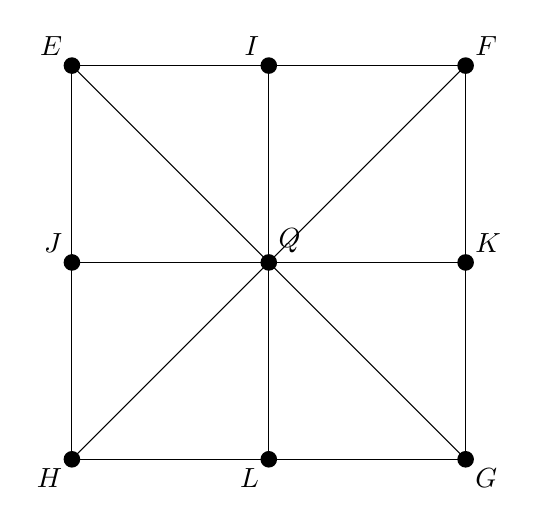
\begin{tikzpicture}
  \coordinate[label=above left:$E$] (E) at (-2.5,2.5);
  \coordinate[label=above right:$F$] (F) at (2.5,2.5);
  \coordinate[label=below right:$G$] (G) at (2.5,-2.5);
  \coordinate[label=below left:$H$] (H) at (-2.5,-2.5);
  \coordinate[label=above left:$I$] (I) at (0,2.5);
  \coordinate[label=above left:$J$] (J) at (-2.5,0);
  \coordinate[label=above right:$K$] (K) at (2.5,0);
  \coordinate[label=below left:$L$] (L) at (0,-2.5);
  \coordinate[label=above right:$Q$] (Q) at (0,0);

  % Draw the inner square
  \draw (E) -- (F) -- (G) -- (H) -- cycle;
  \draw (J)--(Q)--(K);
  \draw (I)--(Q)--(L);
  \draw (E)--(G);
  \draw (H)--(F);

  % Add small points at the inner square vertices
  \foreach \vertex in {E, F, G, H,I,J,K,L,Q}
    \fill (\vertex) circle (3pt);
\end{tikzpicture}
\newpage

\part
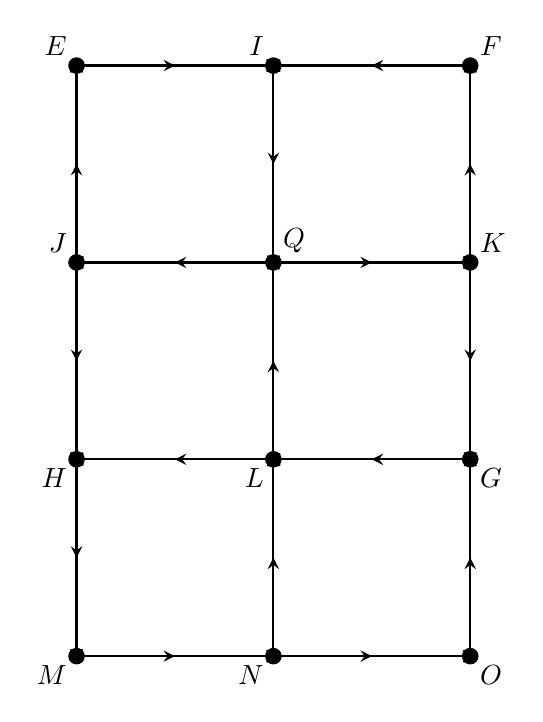
\begin{tikzpicture}
[
  vertex/.style={circle, draw, fill=black, inner sep=3pt},
  arrowmid/.style={postaction=decorate, decoration={
    markings, mark=at position 0.5 with {\arrow{stealth}}}}
  ]
\coordinate[label=above left:$E$] (E) at (-2.5,2.5);
\coordinate[label=above right:$F$] (F) at (2.5,2.5);
\coordinate[label=below right:$G$] (G) at (2.5,-2.5);
\coordinate[label=below left:$H$] (H) at (-2.5,-2.5);
\coordinate[label=above left:$I$] (I) at (0,2.5);
\coordinate[label=above left:$J$] (J) at (-2.5,0);
\coordinate[label=above right:$K$] (K) at (2.5,0);
\coordinate[label=below left:$L$] (L) at (0,-2.5);
\coordinate[label=above right:$Q$] (Q) at (0,0);
\coordinate[label=below left:$M$] (M) at (-2.5,-5);
\coordinate[label=below left:$N$] (N) at (0,-5);
\coordinate[label=below right:$O$] (O) at (2.5,-5);


\foreach \vertex in {E, F, G, H,I,J,K,L,M,N,O,Q}
\fill (\vertex) circle (3pt);

\draw[->, thick, arrowmid] (J) -- (E);
\draw[->, thick, arrowmid] (J) -- (H);
\draw[->, thick, arrowmid] (E) -- (I);
\draw[->, thick, arrowmid] (F) -- (I);
\draw[->, thick, arrowmid] (I) -- (Q);
\draw[->, thick, arrowmid] (L) -- (Q);
\draw[->, thick, arrowmid] (Q) -- (J);
\draw[->, thick, arrowmid] (Q) -- (K);
\draw[->, thick, arrowmid] (K) -- (F);
\draw[->, thick, arrowmid] (K) -- (G);
\draw[->, thick, arrowmid] (H) -- (M);
\draw[->, thick, arrowmid] (M) -- (N);
\draw[->, thick, arrowmid] (N) -- (O);
\draw[->, thick, arrowmid] (O) -- (G);
\draw[->, thick, arrowmid] (N) -- (L);
\draw[->, thick, arrowmid] (G) -- (L);
\draw[->, thick, arrowmid] (L) -- (H);
\end{tikzpicture}
\newpage
\end{parts}

\question . Show that the Petersen graph, shown here, does not have
a Hamilton circuit, but that the subgraph obtained by
deleting a vertex v, and all edges incident with v, does
have a Hamilton circuit.


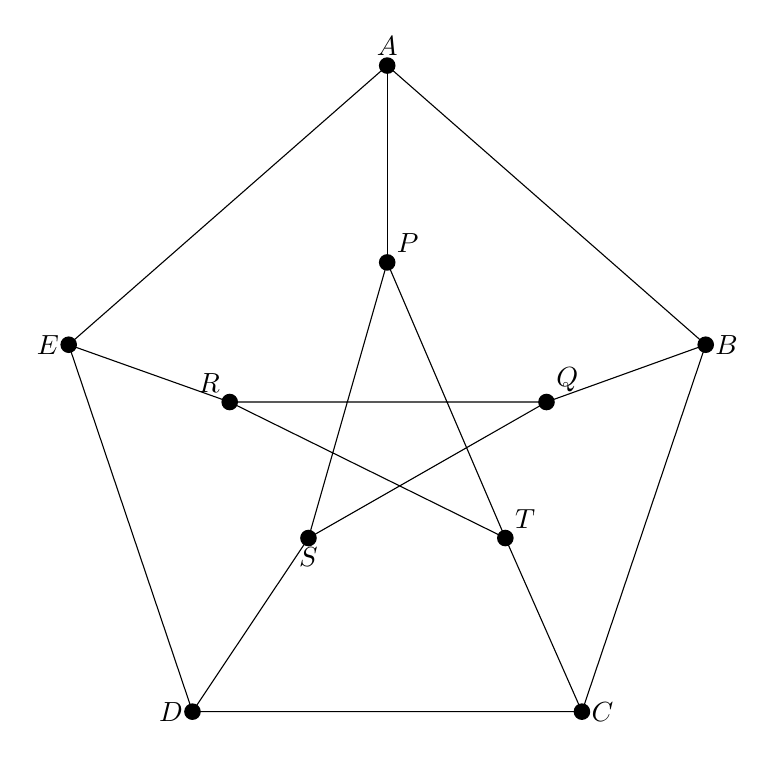
\begin{tikzpicture}
  % Define the coordinates for the vertices of the big pentagon
  \coordinate[label=above:$A$] (A) at (0,5);
  \coordinate[label=right:$B$] (B) at (4.045,1.455);
  \coordinate[label=right:$C$] (C) at (2.473,-3.205);
  \coordinate[label=left:$D$] (D) at (-2.473,-3.205);
  \coordinate[label=left:$E$] (E) at (-4.045,1.455);

  % Draw the big pentagon
  \draw (A) -- (B) -- (C) -- (D) -- (E) -- cycle;

  % Define the coordinates for the vertices of the small pentagon
  \coordinate[label=above right:$P$] (P) at (0,2.5);
  \coordinate[label=above right:$Q$] (Q) at (2.023,0.727);
  \coordinate[label=above left:$R$] (R) at (-2,0.727);
  \coordinate[label=below:$S$] (S) at (-1,-1);
  \coordinate[label=above right:$T$] (T) at (1.5,-1);

  % Draw the small pentagon
  \draw (P) -- (T)--(R)--(Q)--(S)--(P);
  \draw(E)--(R);
  \draw(A)--(P);
  \draw(B)--(Q);
  \draw(T)--(C);
  \draw(S)--(D);
  

  % Add small points at the vertices of both pentagons
  \foreach \vertex in {A, B, C, D, E, P, Q, R, S, T}
    \fill (\vertex) circle (3pt);
\end{tikzpicture}

\end{questions}
\end{document}

